\documentclass[11pt]{article}
\usepackage{fontsize}
\changefontsize{11.5pt}

%====================================================
% 1. Encoding and fonts
%====================================================
\usepackage[T1]{fontenc}
\usepackage[utf8]{inputenc}
\usepackage{microtype}          % better justification, fewer overfull lines

%====================================================
% 2. Page layout and spacing
%====================================================
\usepackage[margin=1in]{geometry}
\usepackage[nodisplayskipstretch]{setspace}
\onehalfspacing
\setlength{\parindent}{0pt}
\setlength{\parskip}{0.25\baselineskip plus 1pt minus 1pt}
\flushbottom

%====================================================
% 3. Mathematics
%====================================================
\usepackage{amsmath}
\allowdisplaybreaks[4]
\usepackage{newtxtext,newtxmath}

% Vertical space around and inside displayed equations
\setlength{\abovedisplayskip}{3pt plus 1pt minus 1pt}
\setlength{\belowdisplayskip}{3pt plus 1pt minus 1pt}
\setlength{\abovedisplayshortskip}{1pt plus 2pt}
\setlength{\belowdisplayshortskip}{2pt plus 2pt minus 1pt}
\setlength{\jot}{3pt}           % row spacing inside align

%====================================================
% 4. Section headings
%====================================================
\usepackage{titlesec}
\titleformat{\section}{\normalfont\large\bfseries}{\thesection}{0.75em}{}
\titleformat{\subsection}{\normalfont\normalsize\bfseries}{\thesubsection}{0.75em}{}
\titlespacing*{\section}{0pt}{8pt plus 2pt minus 2pt}{2pt}
\titlespacing*{\subsection}{0pt}{6pt plus 1pt minus 1pt}{2pt}

%====================================================
% 5. Figures and tables
%====================================================
\usepackage{graphicx}
\usepackage{float}
\usepackage{booktabs}
\usepackage{caption}
\usepackage{etoolbox}

% --- Caption style (applies to all figures and tables) ---
\captionsetup{
  font=small,
  labelfont=bf,
  labelsep=period,
  justification=justified,
  singlelinecheck=true,
  width=0.92\textwidth,
  skip=4pt
}
\captionsetup[table]{position=top, skip=4pt}

% --- Space around floats ---
\setlength{\intextsep}{2pt plus 1pt minus 1pt}
\setlength{\textfloatsep}{1pt plus 2pt minus 2pt}
\setlength{\abovecaptionskip}{0pt}
\setlength{\belowcaptionskip}{0pt}

% --- Compact, evenly spaced tables ---
\AtBeginEnvironment{tabular}{\setstretch{1.0}}
\renewcommand{\arraystretch}{1.15}
\setlength{\tabcolsep}{9pt}

%====================================================
% 6. Bibliography (ACS numbered style)
%====================================================
\usepackage[super,sort&compress,comma]{natbib}
\bibliographystyle{achemso}
\setlength{\bibsep}{2pt plus 1pt}

%====================================================
% 7. Cross-references and hyperlinks (load last)
%====================================================
\usepackage{hyperref}
\hypersetup{hidelinks}

\begin{document}

%====================================================
% Title Block  (counts toward 10-page limit)
%====================================================
\begin{center}
\begingroup
\setstretch{1.15}
{\Large\bfseries
Economic Nonlinear Model Predictive Control with Infinite Horizon for Cyclic Steady State Gas Pipeline Systems\par}

\vspace{10pt}

{\normalsize
Yuming Sun\\[1pt]
Advised by: Larry Biegler, Carl Laird\\[1pt]
July 2026\par}
\endgroup
\end{center}

\vspace{-30pt}

%====================================================
% Abstract  (~300 words, within 10 pages)
%====================================================
\setcounter{secnumdepth}{0}
\section{Abstract}
\setcounter{secnumdepth}{2}

Economic nonlinear model predictive control (eNMPC) has become an effective approach for nonlinear dynamic systems. However, its performance strongly depends on the prediction horizon. Although long prediction horizons reduce suboptimality, they require high computational cost and additional conditions for dynamics beyond the end of finite prediction horizon. To overcome these limitations, we develop an infinite-horizon eNMPC formulation. We extend the formulation to cyclic steady state gas pipeline networks with cyclic customer demand. The proposed formulation consists of a finite prediction horizon followed by an infinite-horizon extension through a time transformation. The infinite-horizon cost is represented by an auxiliary differential equation to avoid the direct evaluation of the infinite integral. Lyapunov-based stability constraints and terminal constraints are used to guarantee closed-loop stability. We implement the formulation on both a test network and the GasLib-40 network. Its performance is evaluated by comparison with finite-horizon eNMPC using short and long finite prediction horizons. As a result, the proposed infinite-horizon eNMPC achieves improved economic performance compared with the short-horizon formulation, and requires 31\% less CPU time than the long-horizon formulation.

%====================================================
% 1.Introduction
%====================================================
\section{Introduction}

Feedback information in closed-loop control systems enables the system to compensate for disturbances and correct deviations. In a closed-loop system, the controller adjusts the manipulated variables (MVs) to drive the control variables (CVs) toward their setpoints. The state variables (SVs) describe the internal dynamics of the plant. There also exist disturbance variables (DVs) to represent external influences.

Model predictive control (MPC) is a widely used closed-loop control strategy. At each sampling time, it uses a dynamic model of the plant to predict future behavior over a horizon, and computes the MVs by solving an optimization problem. Specifically, when the system has nonlinear dynamics, nonlinear model predictive control (NMPC) should be applied. NMPC has a variety of applications. In chemical engineering, NMPC has been applied to improve multivariable control of naphtha distillation units~\cite{STABROV202553} and maximize oil production in wells operated by electrical submersible pumps~\cite{DEABREU2025109304}. Beyond the process industries, NMPC is also widely used in robotics and autonomous vehicles, where it handles trajectory tracking and obstacle avoidance in real time~\cite{11393908,qi2025nmpc}.

Traditional NMPC adopts a tracking objective that minimizes deviations from setpoints. Economic NMPC (eNMPC) instead uses an economic objective to operate the process at its economic optimum~\cite{ELLIS20141156}. However, since the economic cost is generally not positive definite with respect to the state and control variables, additional constraints such as terminal constraints or Lyapunov-based constraints are required to guarantee stability~\cite{5672577,GRIFFITH2018109}. Furthermore, the performance of eNMPC is closely related to the prediction horizon. In general, long prediction horizons reduce suboptimality by better approximating the infinite-horizon optimal control problem~\cite{4639448}. However, with a long prediction horizon, it may require additional conditions on dynamics beyond the end of the finite prediction horizon and can be computationally expensive~\cite{CHEN19981205,DINH2025103565}. To address these limitations, infinite-horizon formulations have been introduced to deal with long-term system behavior without explicitly extending the finite prediction horizon~\cite{keerthi1988}. Quasi-infinite horizon approaches have been developed to approximate the infinite-horizon problem using terminal costs and terminal constraints~\cite{CHEN19981205}. More recently, Dinh et al.~\cite{DINH2025103565} propose an infinite-horizon NMPC formulation that captures long-term system behavior with improved computational efficiency.

Here we extend the infinite-horizon NMPC framework to cyclic steady state systems with economic objectives. Specifically, we develop an infinite-horizon eNMPC formulation for gas pipeline networks with cyclic customer demands. The finite-horizon eNMPC formulation is adopted from Naik et al.~\cite{NAIK2026122276}. Compared with the short finite-horizon formulation, our proposed infinite-horizon eNMPC achieves improved economic performance. It also requires less CPU time than the long finite-horizon formulation.

%====================================================
% 2.ENMPC Control Theory
%====================================================
\section{Cyclic Steady State eNMPC}

\subsection{Cyclic Steady State Calculation}

\begin{figure}[H]
    \centering
    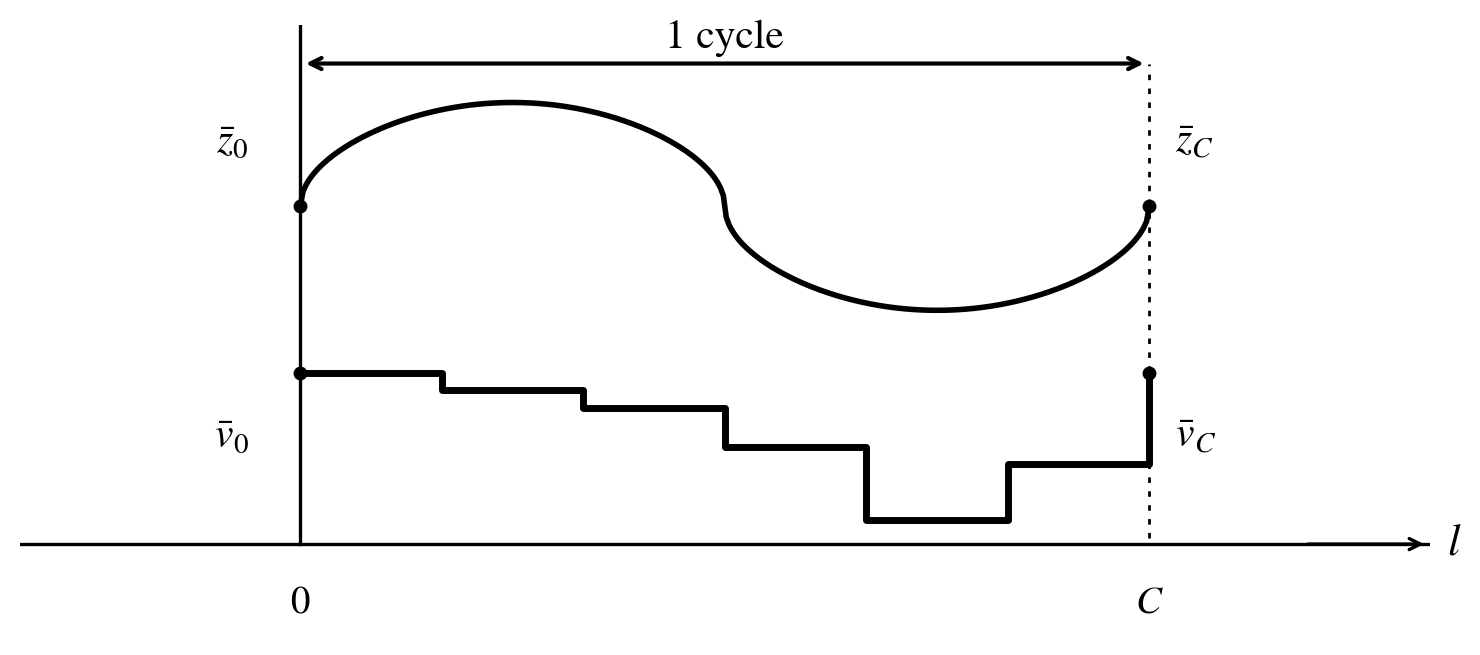
\includegraphics[width=0.5\linewidth]{css_periodicity_sketch.png}
    \caption{Cyclic steady state diagram}
    \label{fig:css}
\end{figure}

This calculation is to determine a cyclic reference for eNMPC. The control objective is to minimize the economic stage cost $\psi^{ec}$ over one-cycle prediction horizon, as shown in Equation~\eqref{eq:enmpc-obj-css}. Equations~\eqref{eq:enmpc-dyn-css}--\eqref{eq:enmpc-alg-css} represent the dynamic equations and inequalities for the system. Equation~\eqref{eq:enmpc-x1-css} makes sure the end conditions are exactly the same as the start conditions. Equation~\eqref{eq:enmpc-bounds-css2} defines the domain for variables.

The cyclic steady state optimization is calculated offline only once. After solving the problem once, we repeat several times to cover the prediction horizon in eNMPC, shown in Figure~\ref{fig:css}. The cycled trajectory of state variable $z$, written as $\bar{z}_{\bar{k}}$, is used as the cyclic steady state reference for eNMPC formulations, where $\bar{z}_{\bar{k}}$ denotes the reference at time step $k$, with $\bar{k} = \operatorname{mod}(k, C)$, $k = 0, 1, 2, \ldots$.
\begin{align}
\min \bar{\Phi}^{ec} &= \sum_{l=0}^{C-1} \psi^{ec}(\bar{z}_l, \bar{v}_l) \label{eq:enmpc-obj-css}\\
\text{s.t.} \quad \bar{z}_{l+1} &= f(\bar{z}_l, \bar{v}_l) \quad l = 0, \ldots, C-1 \label{eq:enmpc-dyn-css}\\
g(\bar{z}_l, \bar{v}_l) &\leq 0 \quad l = 0, \ldots, C-1 \label{eq:enmpc-alg-css}\\
\bar{z}_0 &= \bar{z}_C, \quad \bar{v}_0 = \bar{v}_C \label{eq:enmpc-x1-css}\\
\bar{z}_l &\in X, \quad \bar{v}_l \in U \quad l = 0, \ldots, C \label{eq:enmpc-bounds-css2}
\end{align}

\subsection{Cyclic Steady State eNMPC Formulation}

The basic form of eNMPC is given by Equations~\eqref{eq:enmpc-obj}--\eqref{eq:enmpc-bounds-xf}. The objective function in Equation~\eqref{eq:enmpc-obj} consists of three terms, as illustrated in Figure~\ref{fig:inf_enmpc}. The first term sums the economic stage cost $\psi^{ec}$ over the $N$-cycle finite horizon $N \cdot C$. The second term sums the stage cost $\psi^{ec}$ over the infinite horizon from $l = N \cdot C$ to infinity. The third term $\bar{\Phi}^{ec}$, as in Equation~\eqref{eq:terminal-cost-def}, represents the terminal cost for an additional cycle after the end of the infinite prediction horizon. Since the cyclic steady state reference has been precomputed offline in Equations~\eqref{eq:enmpc-obj-css}--\eqref{eq:enmpc-bounds-css2}, we know the system behavior beyond the prediction horizon, as long as the system reaches the cyclic steady state at the end of the infinite horizon as in Equation~\eqref{eq:terminal-state}. In that case, the system will continue to operate at the cyclic steady state. Under this condition, the terminal cost $\bar{\Phi}^{ec}$ becomes a constant and therefore does not affect the optimization result. As a result, it can be removed from the objective function.
\begin{align}
\min \quad &\sum_{l=0}^{NC-1} \psi^{ec}(z_l, v_l) + \sum_{l=NC}^{\infty} \psi^{ec}(\hat{z}_l, \hat{v}_l) + \bar{\Phi}^{ec} \label{eq:enmpc-obj}\\
\text{s.t.} \quad \bar{\Phi}^{ec} &= \sum_{l=0}^{C-1} \psi^{ec}(\bar{z}_l, \bar{v}_l) \label{eq:terminal-cost-def}\\
z_{l+1} &= f(z_l, v_l), \quad \hat{z}_{l+1} = f(\hat{z}_l, \hat{v}_l) \label{eq:enmpc-dyn}\\
g(z_l, v_l) &\leq 0, \quad g(\hat{z}_l, \hat{v}_l) \leq 0 \label{eq:enmpc-alg}\\
z_0 &= x(k) \label{eq:enmpc-init}\\
\hat{z}_{\infty}(k) &= \bar{z}_{\bar{k}}, \quad \bar{k} = \operatorname{mod}(k, C) \label{eq:terminal-state}\\
z_l, \hat{z}_l, \bar{z}_l &\in X, \quad v_l, \hat{v}_l, \bar{v}_l \in U\label{eq:enmpc-bounds-xf}
\end{align}
Equations~\eqref{eq:enmpc-dyn}--\eqref{eq:enmpc-alg} are equivalent to~\eqref{eq:enmpc-dyn-css}--\eqref{eq:enmpc-alg-css}. The initial condition is given by Equation~\eqref{eq:enmpc-init}, where $k$ is the current sampling time. To guarantee convergence, we should force the system to reach cyclic steady state at the end, as in Equation~\eqref{eq:terminal-state}. Equation~\eqref{eq:enmpc-bounds-xf} defines the domain for variables.

In addition, a Lyapunov-based stability constraint in Equation~\eqref{eq:lyapunov-decay} is enforced to ensure stability. In the infinite horizon formulation, the Lyapunov function is defined as $V(k)$ in Equation~\eqref{eq:lyapunov-def}. It tracks the accumulated deviation from the cyclic steady state reference over the finite prediction horizon $N$ and the remaining infinite horizon. The Lyapunov-based stability constraint ensures that the Lyapunov function decreases monotonically, usually by first-stage cost. The decay rate is decided by the parameter $\delta$.
\begin{align}
V(k) &\leq V(k-1) - \delta\, \psi^{tr}(0), \quad \delta \in (0,1], \quad \text{where} \quad \psi^{tr}(0) = (z_0 - \bar{z}_{\bar{0}})^2 + (v_0 - \bar{v}_{\bar{0}})^2 \label{eq:lyapunov-decay}
\end{align}
\begin{equation}
V(k) = \sum_{l=0}^{NC-1} \left[ (z_l(k) - \bar{z}_{\bar{l}})^2 + (v_l - \bar{v}_{\bar{l}})^2 \right] + \sum_{l=NC}^{\infty} \left[ (\hat{z}_l(k) - \bar{z}_{\bar{l}})^2 + (\hat{v}_l - \bar{v}_{\bar{l}})^2 \right], \bar{l} = \operatorname{mod}(k+l, C) \label{eq:lyapunov-def}
\end{equation}

\begin{figure}[H]
    \centering
    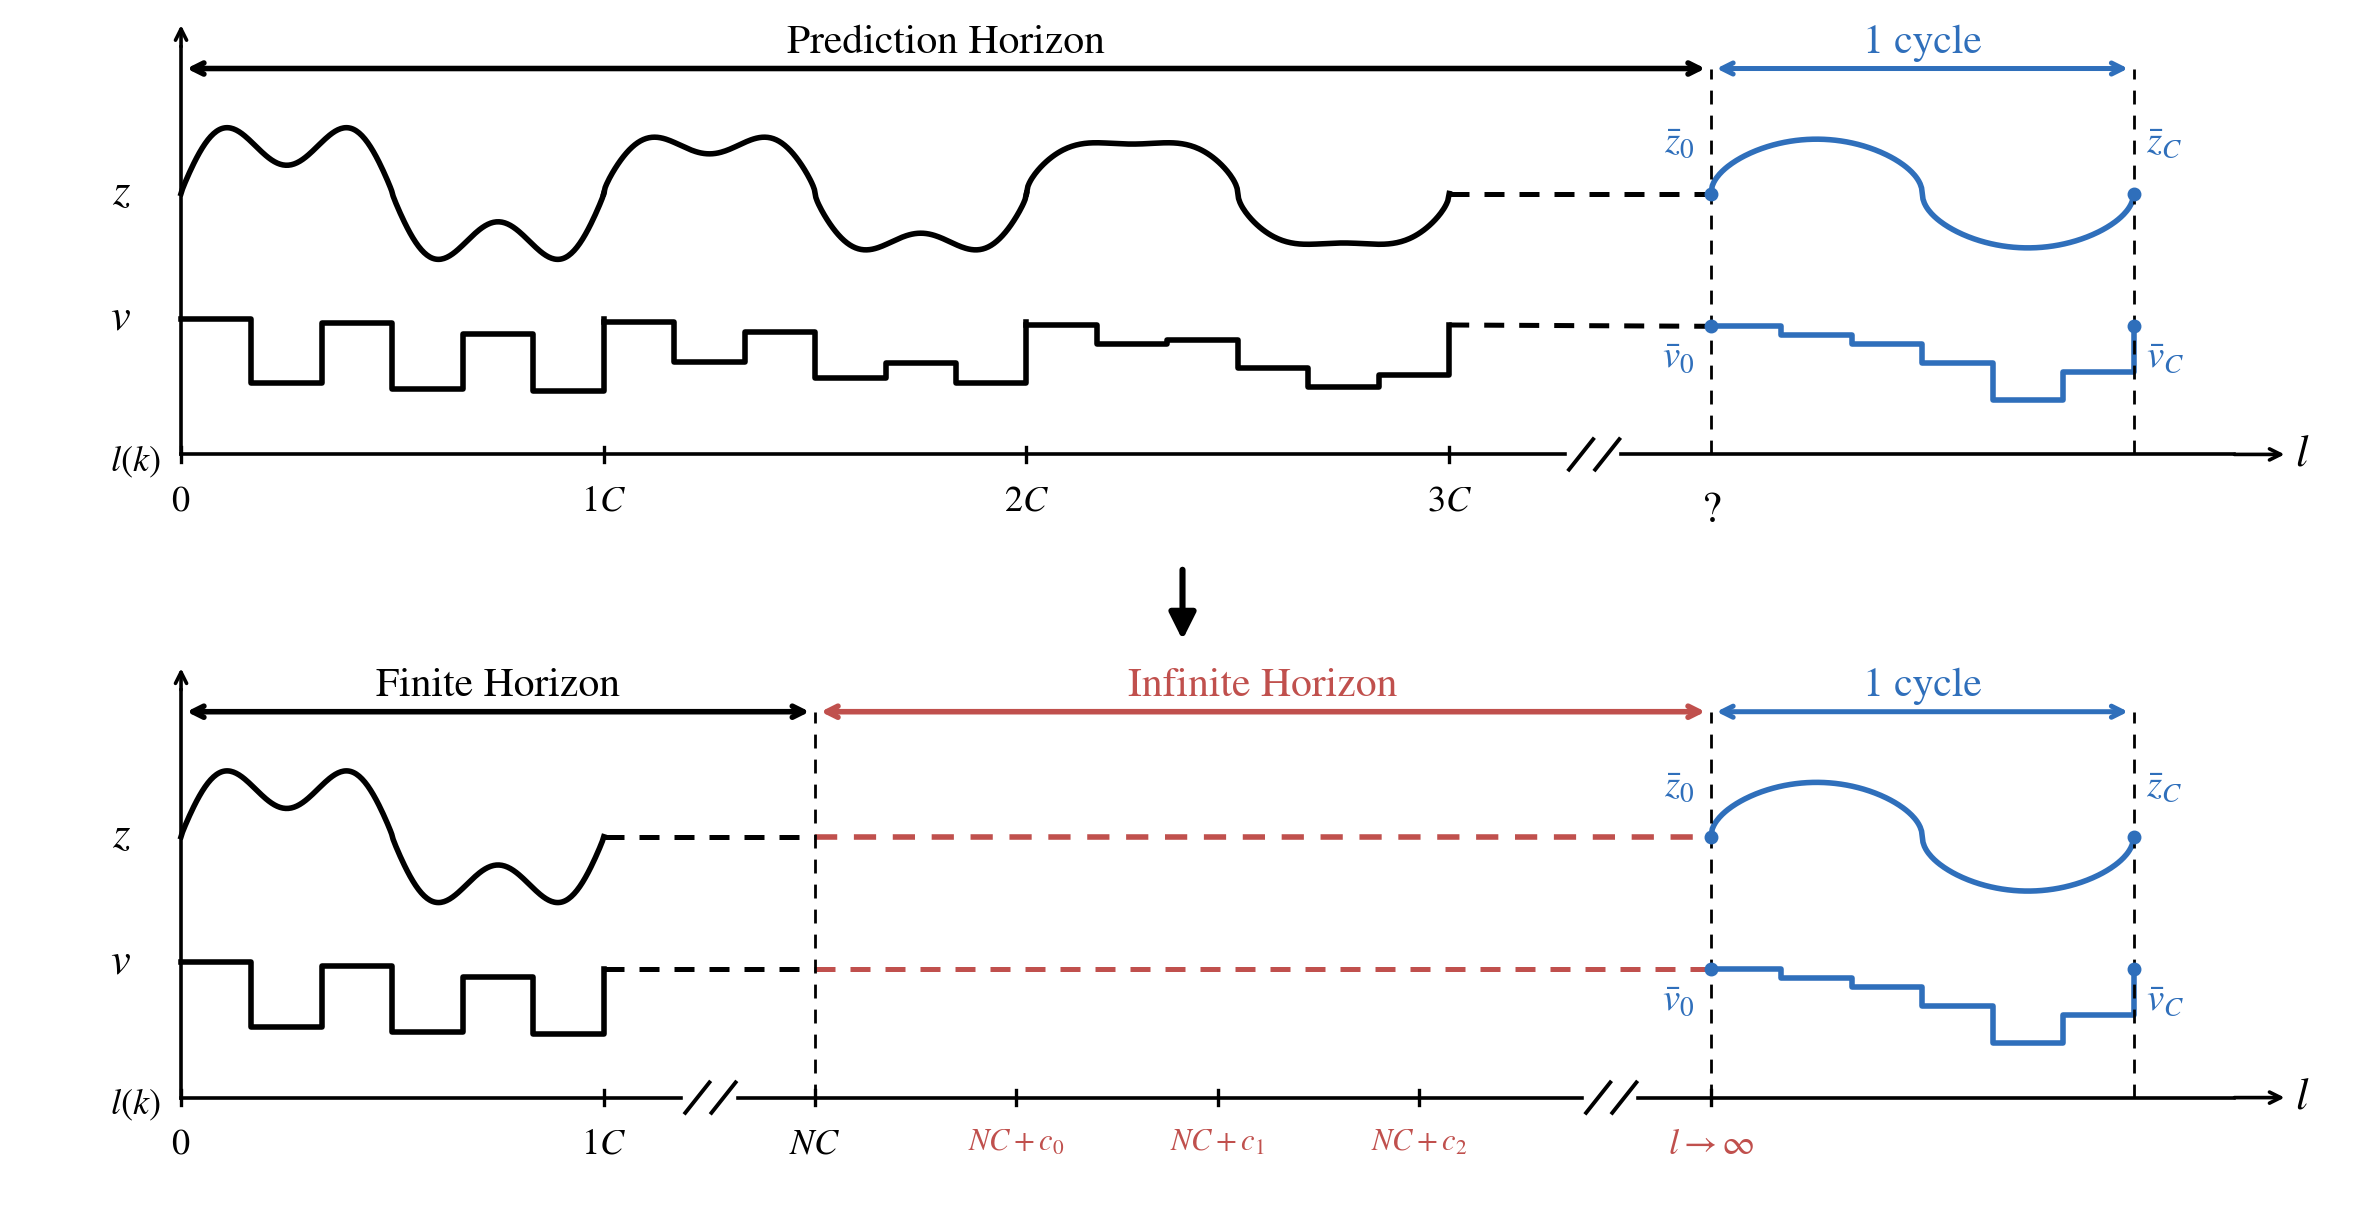
\includegraphics[width=0.8\linewidth]{inf_enmpc.png}
    \caption{Infinite-horizon eNMPC}
    \label{fig:inf_enmpc}
\end{figure}

In summary, the complete cyclic steady state eNMPC formulation is defined by the objective function in Equation~\eqref{eq:enmpc-obj}, subject to the constraints in Equations~\eqref{eq:terminal-cost-def}--\eqref{eq:lyapunov-def}, with the preliminary offline cyclic steady state calculation given by Equations~\eqref{eq:enmpc-obj-css}--\eqref{eq:enmpc-bounds-css2}.

%====================================================
% 3.Model Formulation
%====================================================
\section{Infinite-horizon Formulation}

\subsection{Infinite Time Transformation}

The infinite horizon formulation includes a short period of finite horizon and an infinite extension of time, shown in Figure~\ref{fig:inf_enmpc}. The infinite time transformation is given by Equation~\eqref{eq:time-transform}. $t$ represents continuous time. $\tau$ is the transformed time. $\gamma$ is a decay parameter, which is typically chosen in (0,1). $\Delta t$ is the sampling time of the controller. In this way, the infinite-horizon segment $t\in[NC,\infty)$ is mapped onto the bounded interval $\tau\in[0,1)$.
\begin{equation}
\tau = \tanh\left(\frac{\gamma}{\Delta t}(t - NC)\right) \label{eq:time-transform}
\end{equation}
By the chain rule, the time derivative of variable $x$ is transformed in Equation~\eqref{eq:chain-rule}.
\begin{equation}
\frac{dx}{dt} = \frac{\gamma}{\Delta t}(1-\tau^2)\cdot\frac{dx}{d\tau}
\label{eq:chain-rule}
\end{equation}
\subsection{Objective Function}
The objective function is given by Equation~\eqref{eq:enmpc-obj}. The infinite term in the objective function is shown as an integral in Equation~\eqref{eq:inf-obj}.
\begin{equation}
\hat{\Phi}^{ec} = \frac{1}{\Delta t}\int_{NC}^{\infty} \psi^{ec}(\hat{z}(t), \hat{v}(t))\,dt
\label{eq:inf-obj}
\end{equation}
After transforming $t$ into $\tau$, we have Equation~\eqref{eq:integral-transform}.
\begin{equation}
\hat{\Phi}^{ec} = \frac{1}{\Delta t} \int_0^1 \psi^{ec}(\hat{z}(\tau),\hat{v}(\tau)) \cdot \frac{\Delta t}{\gamma(1-\tau^2)}\,d\tau
= \int_0^1 \frac{\psi^{ec}(\hat{z}(\tau),\hat{v}(\tau))}{\gamma(1-\tau^2)}\, d\tau
\label{eq:integral-transform}
\end{equation}
Rather than computing the integral directly, we reformulate it as a differential equation by defining $\hat{\varphi}^{ec}(\tau)$ as the accumulated infinite horizon cost in Equation~\eqref{eq:varphi-ode}.
\begin{equation}
\gamma(1-\tau^2)\frac{d\hat{\varphi}^{ec}}{d\tau} =\psi^{ec}(\hat{z}(\tau),\hat{v}(\tau)),
\quad \hat{\varphi}^{ec}(0) = 0
\label{eq:varphi-ode}
\end{equation}
Solving Equation~\eqref{eq:varphi-ode} gives Equation~\eqref{eq:Phi-terminal}.
\begin{equation}
\hat{\Phi}^{ec}=\hat{\varphi}^{ec}(1)
\label{eq:Phi-terminal}
\end{equation}
\subsection{Terminal Constraints}
The terminal constraint is given in Equation~\eqref{eq:terminal-css-state}, where $\bar{z}_{\bar{k}}$ is calculated by Equations~\eqref{eq:enmpc-obj-css}--\eqref{eq:enmpc-bounds-css2}.
\begin{align}
\hat{z}(\tau=1, k) &= \bar{z}_{\bar{k}}, \quad \bar{k} = \operatorname{mod}(k, C) \label{eq:terminal-css-state}
\end{align}
\subsection{Stability Constraints}
This accumulated tracking error $\hat{V}(k)$ in Equation~\eqref{eq:Vx} is obtained by the auxiliary differential equation in Equation~\eqref{eq:Vx-ode}. The reference $(\bar{z}(\bar{\tau}), \bar{v}(\bar{\tau}))$ is obtained by interpolating the discrete cyclic steady state reference. The stability constraint
for the Lyapunov function is the same as Equation~\eqref{eq:lyapunov-decay}.
\begin{align}
\hat{V}(k) &= \int_{0}^{1} \frac{1}{\gamma(1-\tau^2)}\left[ (\hat{z}(\tau, k) - \bar{z}(\bar{\tau}))^2 + (\hat{v}(\tau, k) - \bar{v}(\bar{\tau}))^2 \right] \, d\tau \label{eq:Vx}\\
\gamma(1-\tau^2) \frac{d\hat{V}(k)}{d\tau} &= (\hat{z}(\tau, k) - \bar{z}(\bar{\tau}))^2 + (\hat{v}(\tau, k) - \bar{v}(\bar{\tau}))^2, \quad \hat{V}(0) = 0 \label{eq:Vx-ode}
\end{align}
%====================================================
% 4.Model Formulation
%====================================================
\section{Gas Pipeline Infinite-horizon Formulation}

\subsection{Overall Description}

The gas pipeline infinite-horizon model is formulated with objective function in Equation~\eqref{eq:gas-obj}, subject to constraints in Equations~\eqref{eq:gas-phi-ode}--\eqref{eq:gas-stability-2}. For spatial discretization, the pipe partial differential equations in Equations~\eqref{eq:pipe-mass}--\eqref{eq:pipe-eos} are discretized on a staggered finite volume grid. For time discretization, the finite horizon applies backward Euler for its numerical stability and computational efficiency. The infinite horizon applies 3 collocation points on 5 finite elements with Lagrange polynomials on Legendre roots. This selection provides sufficient accuracy to capture the nonlinear dynamics while keeping the problem size tractable. In this gas pipeline control problem, gas density, pipe pressure, gas flow rate, and compressor power are the state variables that change with time. Compression ratio is the manipulated variable. This infinite time formulation is an extension of the finite horizon formulation by Naik et al.~\cite{NAIK2026122276}.

\subsection{Cyclic Steady State Calculation}

The objective of the cyclic steady state reference calculation is given in Equation~\eqref{eq:css-obj}. It minimizes the total compression power over one cycle. The dynamic constraints are shown in Equations~\eqref{eq:pipe-mass}--\eqref{eq:comp-bounds}.
\begin{align}
\min \bar{\Phi}^{ec} &= \sum_{l=0}^{C-1} \sum_{c \in \mathcal{C}} P_{c,l} \label{eq:css-obj}
\end{align}
To obtain a cyclic steady state solution, periodic conditions are imposed by requiring the pipe pressure and compressor power at the beginning of the cycle to be equal to those at the end of the cycle, as in Equations~\eqref{eq:enmpc-x-css}--\eqref{eq:enmpc-u-css}.
\begin{align}
p_0 &= p_C \label{eq:enmpc-x-css}\\
P_{c,0} &= P_{c,C}, \quad \forall c \in \mathcal{C} \label{eq:enmpc-u-css}
\end{align}

\subsection{Objective Function}

The objective minimizes the total compression power $P_{c,l}$ over both finite and infinite horizons, as formulated in Equation~\eqref{eq:gas-obj}. The finite-horizon component sums the compressor power over the sampling intervals. The infinite-horizon component $\hat{\varphi}^{ec}_{\tau=1}$ is obtained from Equation~\eqref{eq:gas-phi-ode}, where $\gamma$ is a decay parameter.
\begin{align}
\min \Phi^{ec} &= \sum_{l=0}^{NC-1} \sum_{c \in \mathcal{C}} P_{c,l} + 、\hat{\varphi}^{ec}_{\tau=1} \label{eq:gas-obj} \\
\gamma(1-\tau^2)\frac{d\hat{\varphi}^{ec}}{d\tau} &= \sum_{c \in \mathcal{C}} P_{c,\tau} \quad \hat{\varphi}^{ec}(0) = 0 \label{eq:gas-phi-ode}
\end{align}

\subsection{Gas Pipeline Constraints}

The mathematical model with nonlinear dynamics for the gas pipeline network is formulated according to Ghilardi et al.~\cite{GHILARDI2024}. The definitions of the variables, parameters, and sets are summarized in Table~\ref{tab:nomenclature} in Appendix. Equation~\eqref{eq:pipe-mass} is pipe mass balance. Equation~\eqref{eq:pipe-momentum} is pipe momentum balance. Equation~\eqref{eq:gas-velocity} describes the gas velocity. Equation~\eqref{eq:pipe-eos} describes the gas state, where $Z$ is a compressibility factor.
\begin{align}
\frac{\partial \rho}{\partial t} + \frac{\partial(\rho s)}{\partial L} &= 0 \label{eq:pipe-mass} \\
\frac{\partial p}{\partial L} + \frac{c_f}{2D}\rho|s|s &= 0 \label{eq:pipe-momentum} \\
s &= \frac{w}{\rho A} \label{eq:gas-velocity}\\
p &= Z\frac{\rho RT}{MW} \label{eq:pipe-eos}
\end{align}
Equation~\eqref{eq:node-mass} is mass balance for node $n$. Equation~\eqref{eq:node-bounds} represents the upper and lower bounds on nodes.
\begin{align}
\sum_{a \in IN(n)} w_{a,l}^{\text{out}} + w_{n,l}^{\text{supply}} &= \sum_{a \in OUT(n)} w_{a,l}^{\text{in}} + w_{n,l}^{\text{cons}}
\quad \forall n \in \mathcal{N}, \forall l = 0,1,2,\dots \label{eq:node-mass} \\
p_n^{\text{LB}} \leq p_{n,l} &\leq p_n^{\text{UB}} \quad \forall n \in \mathcal{N}, \forall l = 0,1,2,\dots \label{eq:node-bounds}
\end{align}
Equation~\eqref{eq:comp-mass} is compressor mass balance, and Equation~\eqref{eq:comp-boost} represents the compressor boost rule. Compressor power is calculated by Equation~\eqref{eq:comp-power}. Equation~\eqref{eq:comp-bounds} shows the bounds on $\beta_{c,l}$.
\begin{align}
w_{c,l}^{\text{in}} &= w_{c,l}^{\text{out}} \quad \forall c \in \mathcal{C}, \forall l = 0,1,2,\dots \label{eq:comp-mass} \\
\beta_{c,l} &= \frac{p_{c,l}^{\text{out}}}{p_{c,l}^{\text{in}}} \quad \forall c \in \mathcal{C}, \forall l = 0,1,2,\dots \label{eq:comp-boost} \\
P_{c,l} &= \frac{w_{c,l}^{\text{in}} \cdot c_p \cdot T_{\text{in}} \cdot (\beta_{c,l}^{\theta} - 1)}{\eta} \quad \forall c \in \mathcal{C}, \forall l = 0,1,2,\dots \label{eq:comp-power} \\
\beta_c^{\text{LB}} \leq \beta_{c,l} &\leq \beta_c^{\text{UB}} \quad \forall c \in \mathcal{C}, \forall l = 0,1,2,\dots \label{eq:comp-bounds}
\end{align}

\subsection{Initial Conditions and Terminal Constraints}

At each sampling instant, the optimization is initialized from the current system state. Therefore, the initial pipe pressure is fixed to the measured pressure, as shown in Equation~\eqref{eq:gas-initial}.
\begin{align}
p_0 &= p(k) \label{eq:gas-initial}
\end{align}
To ensure convergence, the terminal pipe pressure is constrained to the corresponding cyclic steady state reference obtained from the offline cyclic steady state calculation, as in Equation~\eqref{eq:gas-terminal}. The reference is calculated in Equations~\eqref{eq:css-obj}--\eqref{eq:enmpc-u-css} and Equations~\eqref{eq:pipe-mass}--\eqref{eq:comp-bounds}. 
\begin{align}
p_{\tau=1} &= \bar{p}_{\bar{k}}, \qquad \bar{k}=\operatorname{mod}(k,C) \label{eq:gas-terminal}
\end{align}

\subsection{Stability Constraints}

The Lyapunov function is defined in Equation~\eqref{eq:gas-Vx}. The reference pressure $\bar{p}_{\bar{l}}$, $\bar{p}_{\bar{\tau}}$ and reference compression ratio $\bar{\beta}_{c,\bar{l}}$, $\bar{\beta}_{c,\bar{\tau}}$ are both obtained from the offline cyclic steady state calculation. $\sigma_p$, $\hat{\sigma}_p$, $\sigma_b$, and $\hat{\sigma}_b$ are scaling weights to balance tracking errors between finite and infinite horizons. $\gamma$ is a decay parameter. For the infinite component, the accumulated tracking error is computed through the auxiliary differential equation in Equations~\eqref{eq:gas-phiVp-ode}--\eqref{eq:gas-phiVb-ode}. Here, the infinite-horizon reference $(\bar{p}_{\bar{\tau}}, \bar{\beta}_{c,\bar{\tau}})$ is obtained by interpolating the discrete cyclic steady state reference $(\bar{p}_{\bar{l}}, \bar{\beta}_{c,\bar{l}})$ onto the transformed time $\tau$.
\begin{equation}
V(k) = \sum_{l=0}^{NC-1} \left[ \frac{(p_l - \bar{p}_{\bar{l}})^2}{\sigma_p} + \sum_{c \in \mathcal{C}}\frac{(\beta_{c,l} - \bar{\beta}_{c,\bar{l}})^2}{\sigma_b} \right] + \frac{\hat{V}^{p}_{\tau=1}}{\hat{\sigma}_p} + \frac{\hat{V}^{\beta}_{\tau=1}}{\hat{\sigma}_b}, \quad \bar{l} = \operatorname{mod}(k+l, C) \label{eq:gas-Vx}
\end{equation}
\begin{align}
\gamma(1-\tau^2) \frac{d\hat{V}^{p}}{d\tau} &= (\hat{p}_\tau - \bar{p}_{\bar{\tau}})^2, \quad \hat{V}^{p}(0) = 0 \label{eq:gas-phiVp-ode}\\
\gamma(1-\tau^2) \frac{d\hat{V}^{\beta}}{d\tau} &= \sum_{c \in \mathcal{C}}(\hat{\beta}_{c,\tau} - \bar{\beta}_{c,\bar{\tau}})^2, \quad \hat{V}^{\beta}(0) = 0 \label{eq:gas-phiVb-ode}
\end{align}
We apply two-phase stability constraints at each rolling horizon step in Equation~\eqref{eq:gas-stability-1} and~\eqref{eq:gas-stability-2}. $\delta$ and $\delta'$ are parameters. $\psi^{tr}(0)$ is defined in Equation~\eqref{eq:lyapunov-decay}. The Lyapunov function first decreases by a percentage of its current value and then transitions to decreasing by the first stage cost of the controller. This two-phase design addresses the initial slow convergence problem.
\begin{align}
V(k) &\leq V(k-1) - \delta\, V(k-1), \quad \delta \in (0,1], \quad k = 1, \ldots, K \label{eq:gas-stability-1} \\
V(k) &\leq V(k-1) - \delta'\, \psi^{tr}(0), \quad \delta' \in (0,1], \quad k = K+1, \ldots \label{eq:gas-stability-2}
\end{align}

%====================================================
% 5.Problem Statement
%====================================================
\section{Pipeline Case Studies}

\subsection{Pipeline Description}

Figure~\ref{fig:network-topology} illustrates (a) the test network with 9 nodes and (b) GasLib-40 with 40 nodes~\cite{gaslib_website}. The pipeline sources should have either fixed pressure or fixed flow rate~\cite{zavala2014stochastic}. After being introduced at sources, the gas is compressed in compressor stations and transported to customers. At customer nodes, there is a minimum delivery pressure. In this study, we define the customer demand as a cyclic pattern. The objective is to minimize total compressor power over all compressor stations. Meanwhile, we must meet customer demand and ensure the system reaches cyclic steady state.

\begin{figure}[htbp]
    \centering
    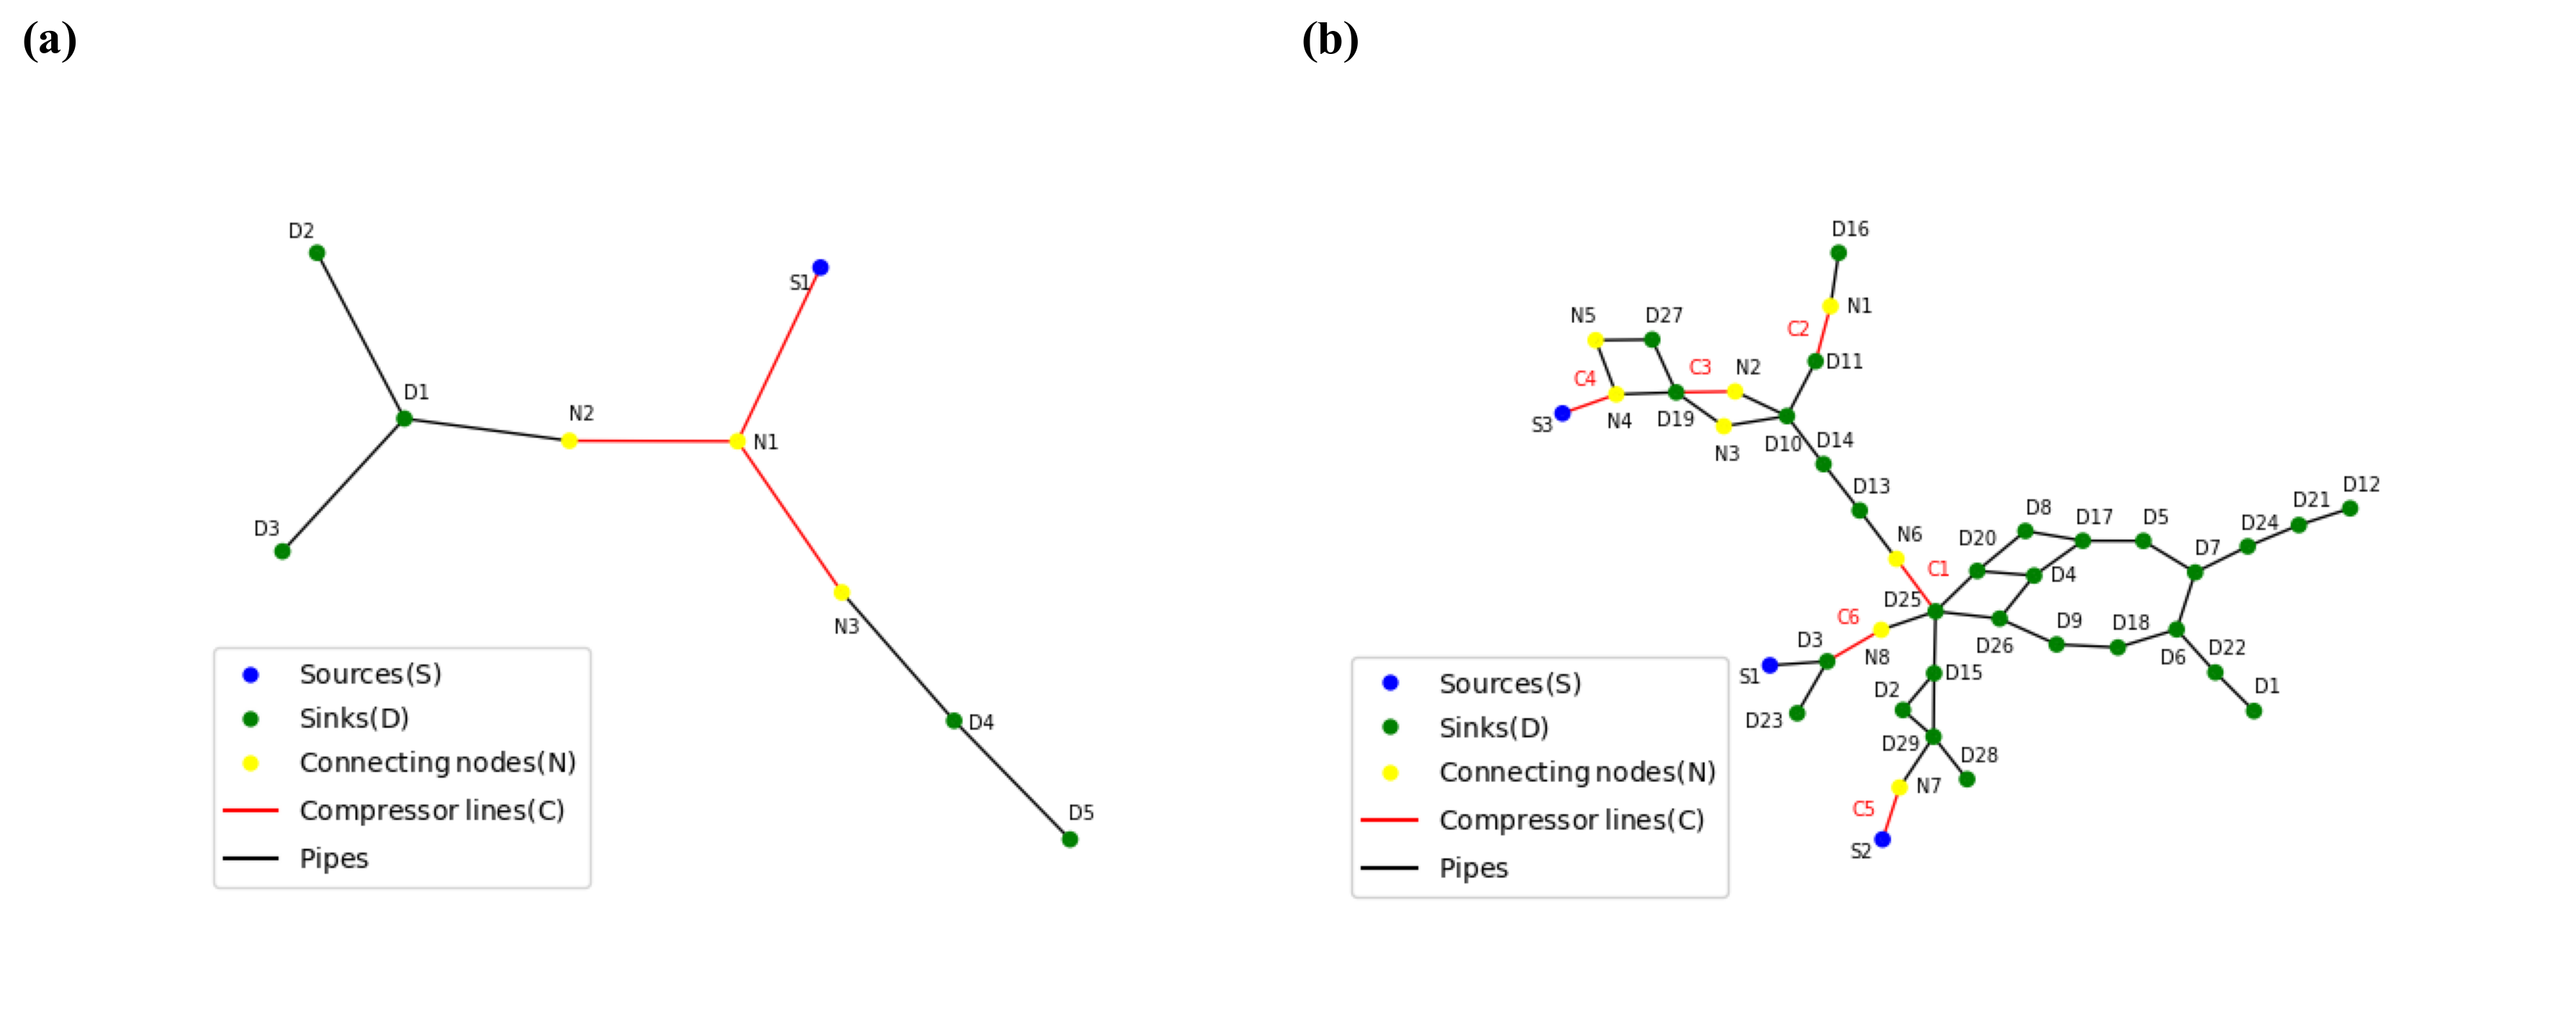
\includegraphics[width=\linewidth, height=0.25\textheight, keepaspectratio]{problem_statement.png}
    \caption{Gas pipeline network}
    \label{fig:network-topology}
\end{figure}

\subsection{Test Network}

In the test example, there is only one source with fixed pressure (Figure~\ref{fig:test-results}). The customer demand follows a staged profile that repeats every 6 hours. The plant is simulated for 4 cycles with 24 hours. All three controllers converge to the cyclic steady state after roughly 2 cycles. Once the system reaches cyclic steady state, it stays on the cyclic steady state trajectory as the simulation time is extended.

\begin{figure}[htbp]  
    \centering
    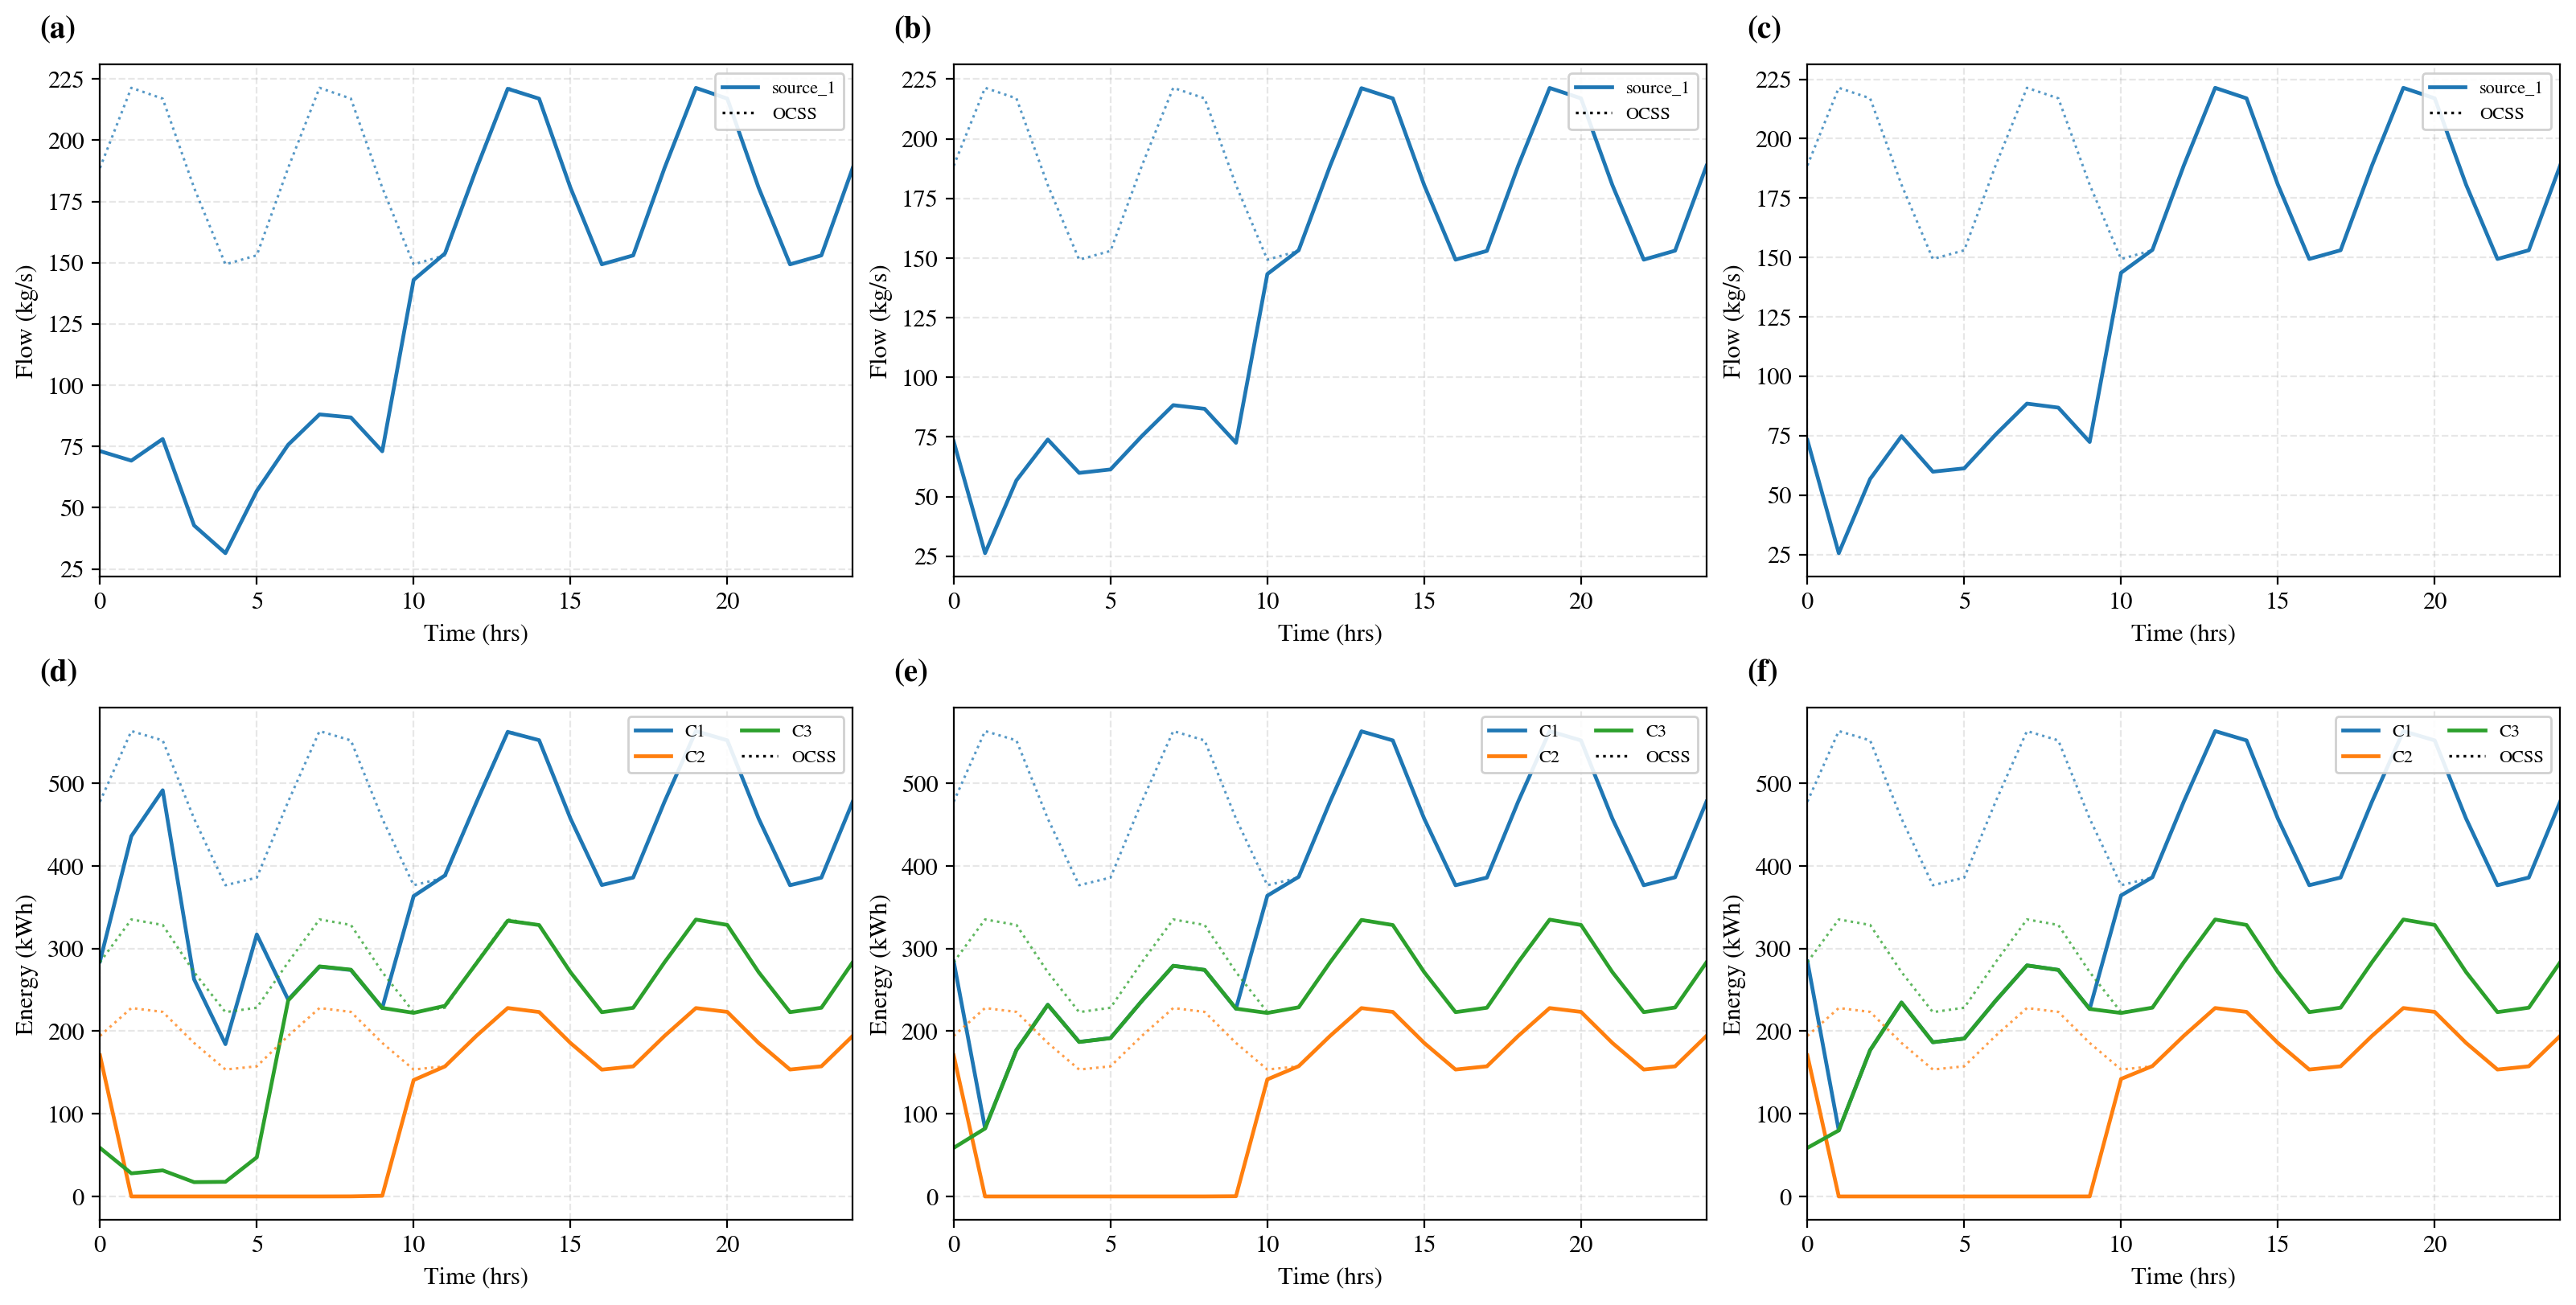
\includegraphics[width=0.8\linewidth]{enmpc_comparison_paper.png}
    \caption{Source flow rate for test network by eNMPC with (a) 1-cycle finite horizon, (b) 10-cycle finite horizon, and (c) infinite horizon with 1-cycle finite segment; Energy consumption for eNMPC with (d) 1-cycle finite horizon, (e) 10-cycle finite horizon, and (f) infinite horizon with 1-cycle finite segment}
    \label{fig:test-results}
\end{figure}

As shown in Table~\ref{tab:test-performance}, from the aspect of economic performance, the infinite-horizon eNMPC achieves the same objective value as the long-horizon eNMPC, with both outperforming the short-horizon eNMPC. From the aspect of computational efficiency, the infinite-horizon eNMPC achieves an 18\% reduction in CPU time compared with the long-horizon eNMPC.

\vspace{8pt}     
\begin{table}[H]
    \centering
    \caption{Model size and performance for the test network.}
    \label{tab:test-performance}
    \begin{tabular}{lccc}
        \toprule
         & 1-cycle & 10-cycle & Infinite \\
        \midrule
        Variables       & 852   & 7,428 & 3,360 \\
        Constraints     & 834   & 7,260 & 3,239 \\
        Objective (kWh) & 5,024 & 4,998 & 4,998 \\
        CPU time (s)    & 7     & 38    & 31    \\
        \bottomrule
    \end{tabular}
\end{table}

The 1-cycle horizon eNMPC is the least computationally expensive to solve, but its prediction horizon is too short to provide sufficient optimization flexibility. As a result, the controller tends to prioritize constraint satisfaction in the early stages at the expense of economic performance. In contrast, the 10-cycle horizon eNMPC provides more degrees of freedom and therefore achieves a lower objective value as 4,998 kWh. However, this improvement comes with a substantially larger optimization problem, containing 7,260 constraints and requiring 38~s of total computation time because the entire 10-cycle prediction horizon must be discretized. The infinite-horizon formulation retains the same economic performance while replacing the final 9 demand cycles with a single transformed infinite horizon, reducing the problem size to 3,239 constraints and the total computation time to 31~s.

\subsection{GasLib-40 Network}

Figure~\ref{fig:GasLib-40-results} shows the source pressure, flow rate, and energy consumption for the GasLib-40 network. In this example, source 1 and 2 have fixed pressure, and source 3 has fixed flow rate. The customer demand follows a sinusoidal profile with a 24-hour period. The plant is simulated for 3 cycles. These 3 eNMPCs have similar performance. A larger network carries more linepack (i.e., pipeline capacitance), which buffers the initial transient, so the system converges to cyclic steady state within one cycle.

\begin{figure}[htbp]  
    \centering
    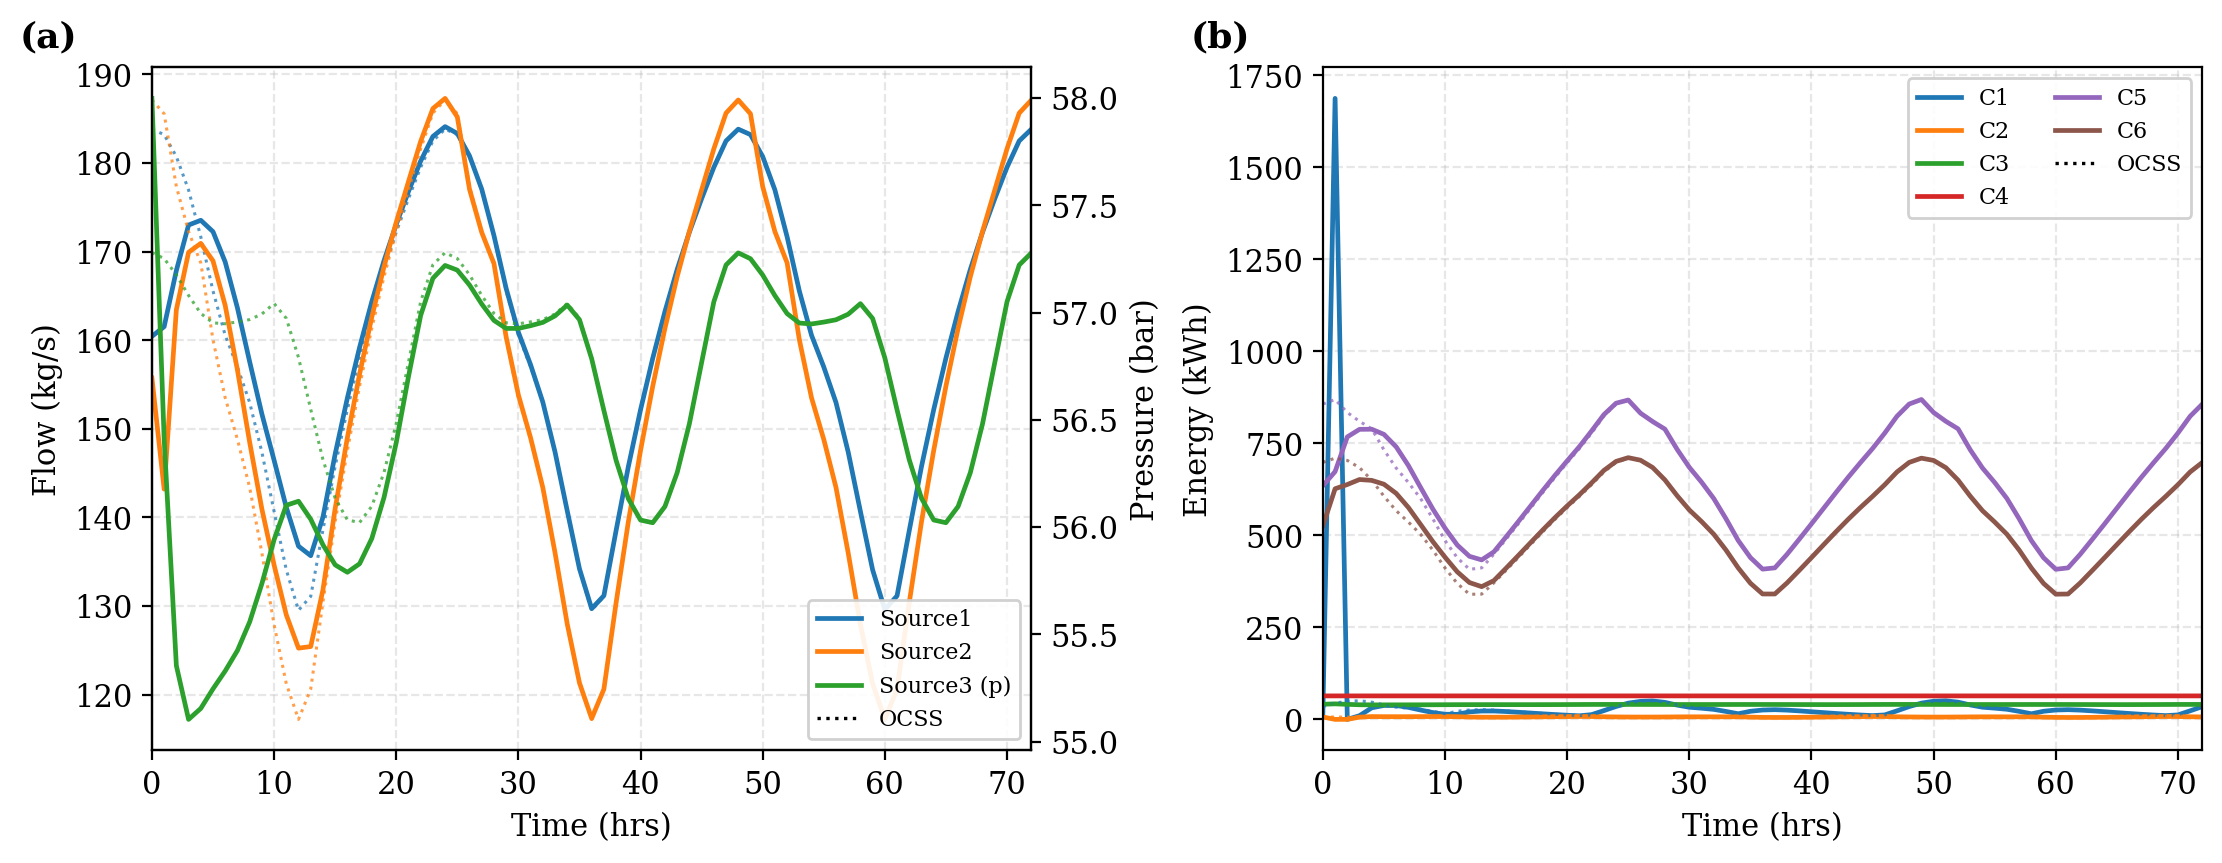
\includegraphics[width=0.7\linewidth]{enmpc_comparison_paper_gaslib40.png}
    \caption{eNMPCs results with 1-cycle finite horizon, 10-cycle finite horizon, and infinite horizon with 1-cycle finite segment: (a) Source pressure and flow rate for GasLib-40 network (b) Energy consumption}
    \label{fig:GasLib-40-results}
\end{figure}

Table~\ref{tab:GasLib-40-performance} further demonstrates the advantage of the infinite-horizon formulation on this larger network. The infinite-horizon eNMPC reduces the total CPU time by 31\% compared with the long-horizon eNMPC, highlighting its computational efficiency.

\vspace{8pt}     
\begin{table}[H]
    \centering
    \caption{Model size and performance for the GasLib-40 network.}
    \label{tab:GasLib-40-performance}
    \begin{tabular}{lccc}
        \toprule
         & 1-cycle & 10-cycle & Infinite \\
        \midrule
        Variables       & 21,176 & 204,011 & 38,172 \\
        Constraints     & 20,909 & 202,682 & 37,764 \\
        Objective (kWh) & 27,165 & 27,165  & 27,164 \\
        CPU time (s)    & 619    & 11,515  & 7,907  \\
        \bottomrule
    \end{tabular}
\end{table}
\vspace{-5pt} 

%====================================================
% 7. Conclusion
%====================================================
\section{Conclusion and Future Work}

We present an infinite-horizon eNMPC formulation for cyclic steady state gas pipeline network systems with cyclic customer demand. The proposed formulation combines a finite prediction horizon with an infinite-horizon extension through a time transformation. It maintains closed-loop stability using Lyapunov-based stability constraints and terminal constraints. Results on both a test network and the GasLib-40 network demonstrate that the infinite-horizon formulation achieves better economic performance than the short-horizon formulation, and less computational time than the long-horizon formulation. These results indicate that the proposed approach is well-performed for real-time economic control of large-scale cyclic gas pipeline network systems. For future work, there are 3 main directions: 1) Address eNMPC for larger pipeline networks, e.g., GasLib-135, 2) Integrate network eNMPC with processing plants, 3) Explore robust eNMPC under uncertainty.

%====================================================
% AI/LLM Statement  (within 10-page limit)
%====================================================
\section*{Statement on AI/LLM Usage}

I use Claude, ChatGPT, and Gemini to help generate some figures, format equations in LaTeX and polish my words. They also help to organize notations in the Appendix. I use Claude Code and Codex to explain Sakshi's code and Owen's code. They also assist in generating an initial version of the infinite-horizon gas pipeline formulation. Based on this version, I rewrite all of the code.

%====================================================
% Appendix
%====================================================
\newpage
\section*{Appendix}

{\renewcommand{\arraystretch}{1.0}          
\begin{table}[H]
\centering
\caption{Notation used in the gas pipeline formulation.}
\label{tab:nomenclature}
\begin{tabular}{@{}ll@{}}
\toprule
\multicolumn{2}{@{}l}{\textbf{Sets}}\\
\midrule
$\mathcal{N}$ & Set of nodes \\
$\mathcal{C}$ & Set of compressors \\
$IN(n)$ & Set of pipelines entering node $n$ \\
$OUT(n)$ & Set of pipelines leaving node $n$ \\
\midrule
\multicolumn{2}{@{}l}{\textbf{Variables}}\\
\midrule
$\rho$ & Gas density \\
$s$ & Gas velocity \\
$p$ & Gas pressure \\
$w_{a,l}^{\mathrm{in}}$ & Mass flow entering pipeline $a$ at step $l$ \\
$w_{a,l}^{\mathrm{out}}$ & Mass flow leaving pipeline $a$ at step $l$ \\
$w_{n,l}^{\mathrm{supply}}$ & Gas supply at node $n$ at step $l$ \\
$w_{n,l}^{\mathrm{cons}}$ & Gas demand at node $n$ at step $l$ \\
$p_{n,l}$ & Pressure at node $n$ at step $l$ \\
$w_{c,l}^{\mathrm{in}}$ & Compressor inlet mass flow \\
$w_{c,l}^{\mathrm{out}}$ & Compressor outlet mass flow \\
$p_{c,l}^{\mathrm{in}}$ & Compressor inlet pressure \\
$p_{c,l}^{\mathrm{out}}$ & Compressor outlet pressure \\
$\beta_{c,l}$ & Compressor pressure ratio \\
$P_{c,l}$ & Compressor power \\
\midrule
\multicolumn{2}{@{}l}{\textbf{Parameters}}\\
\midrule
$L$ & Axial coordinate along the pipeline \\
$D$ & Pipe diameter \\
$A$ & Pipe cross-sectional area \\
$c_f$ & Pipe friction factor \\
$Z$ & Gas compressibility factor \\
$R$ & Universal gas constant \\
$MW$ & Molecular weight of gas \\
$T$ & Temperature \\
$T_{\mathrm{in}}$ & Compressor inlet gas temperature \\
$c_p$ & Specific heat capacity of gas \\
$\eta$ & Compressor efficiency \\
$\theta$ & Compressor power exponent \\
$p_n^{\mathrm{LB}}$ & Minimum pressure at node $n$ \\
$p_n^{\mathrm{UB}}$ & Maximum pressure at node $n$ \\
$\beta_c^{\mathrm{LB}}$ & Minimum compressor pressure ratio \\
$\beta_c^{\mathrm{UB}}$ & Maximum compressor pressure ratio \\
\bottomrule
\end{tabular}
\end{table}
}
%====================================================
% Bibliography  (outside page count, no page limit)
%====================================================
\newpage
\bibliography{references}

\end{document}